\documentclass[10pt, a4paper, twosize]{article}
%\documentclass[12pt, a4paper, twoside]{book}

\usepackage{helvet}
\usepackage{hyperref}
\usepackage{graphicx}
\usepackage{listings}
\usepackage{textcomp}
\usepackage[
	a4paper,
	outer=2cm,
	inner=4cm,
	top=2cm,
	bottom=2cm
]{geometry}
\usepackage{float}
\usepackage{tabularx}
\usepackage[disable]{todonotes}
\usepackage{color, soul}
\usepackage{amsmath}
\usepackage{algorithmicx}
\usepackage[noend]{algpseudocode}
\usepackage{algorithm}
\usepackage{framed}
\usepackage{subcaption}
\usepackage{titlepic}
\usepackage{fancyhdr}
\usepackage[simplified]{styles/pgf-umlcd}
\usepackage{shorttoc}
\usepackage{url}
\usepackage{paralist}

\definecolor{grey}{rgb}{0.9, 0.9, 0.9}
\definecolor{dkgreen}{rgb}{0,0.6,0}
\definecolor{dkred}{rgb}{0.6,0,0.0}

\lstdefinestyle{DOS}
{
    backgroundcolor=\color{black},
    basicstyle=\scriptsize\color{white}\ttfamily,
    stringstyle=\color{white},
    keywords={}
}

\lstdefinestyle{makefile}
{
    numberblanklines=false,
    language=make,
    tabsize=4,
    keywordstyle=\color{red},
    identifierstyle= %plain identifiers for make
}

\lstset{
  language=Java,                % the language of the code
  basicstyle=\footnotesize\ttfamily,
  numbers=left,                   % where to put the line-numbers
  stepnumber=1,                   % the step between two line-numbers. If it's 1, each line
  numbersep=5pt,                  % how far the line-numbers are from the code
  backgroundcolor=\color{white},      % choose the background color. You must add \usepackage{color}
  showspaces=false,               % show spaces adding particular underscores
  showstringspaces=false,         % underline spaces within strings
  showtabs=false,                 % show tabs within strings adding particular underscores
  frame=single,                   % adds a frame around the code
  rulecolor=\color{black},        % if not set, the frame-color may be changed on line-breaks within not-black text (e.g. comments (green here))
  tabsize=2,                      % sets default tabsize to 2 spaces
  captionpos=b,                   % sets the caption-position to bottom
  breaklines=true,                % sets automatic line breaking
  breakatwhitespace=false,        % sets if automatic breaks should only happen at whitespace
  keywordstyle=\color{blue},          % keyword style
  commentstyle=\color{dkgreen},       % comment style
  stringstyle=\color{dkred},         % string literal style
  columns=fixed,
  extendedchars=true,
  frame=single,
}

%\renewcommand{\chaptername}{Topic}

% New definitions
\algnewcommand\algorithmicswitch{\textbf{switch}}
\algnewcommand\algorithmiccase{\textbf{case}}
\algnewcommand\algorithmicassert{\texttt{assert}}
\algnewcommand\Assert[1]{\State \algorithmicassert(#1)}%
% New "environments"
\algdef{SE}[SWITCH]{Switch}{EndSwitch}[1]{\algorithmicswitch\ #1\ \algorithmicdo}{\algorithmicend\ \algorithmicswitch}%
\algdef{SE}[CASE]{Case}{EndCase}[1]{\algorithmiccase\ #1}{\algorithmicend\ \algorithmiccase}%
\algtext*{EndSwitch}%
\algtext*{EndCase}%

\pagestyle{fancy}
\fancyhf{}
\fancyhead[RO, LE]{\small \rightmark}
\fancyfoot[RO, LE]{\small \thepage}

\begin{document}

%\frontmatter

\begin{titlepage}
\vspace*{5cm}
\begin{center}

\includegraphics[width=.5\textwidth]{images/EdNapUniLogoCMYK}~\\[1cm]

\textsc{\Large Edinburgh Napier University}\\[1.5cm]

\textsc{\LARGE \bfseries \LaTeX}\\[0.5cm]

\hrulefill \\[0.4cm]
{\huge \bfseries Quick Start \\[0.4cm] }
\hrulefill \\[1.5cm]

\begin{minipage}{0.4\textwidth}
\begin{flushleft} \large
\textbf{Dr Simon Wells} \\
\end{flushleft}
\end{minipage}

\vfill

\end{center}
\end{titlepage}

%\shorttoc{Overview}{0}

%\setcounter{tocdepth}{2}
%\cleardoublepage
%\tableofcontents
%\listoffigures
%\listofalgorithms
%\addtocontents{toc}{~\hfill\textbf{Page}\par}

%\mainmatter

%\input{sections/labs/04_ui}

\section{Introduction}
\paragraph{} The aim of this quick start is to go from zero to your first report written using \LaTeX and the Napier report template.

\paragraph{} Many of you will be familiar with word processing tools. These are very useful for \emph{ad hoc} documents but are poor for type-setting. There are many professional type setting tools available, but \LaTeX is one that is particulaly good for academic typesetting; creating documents that may contain mathematical formulae, programming source code, algortihms, images, and many other things that are frustrating to work with in a word processor.

\paragraph{} The idea with \LaTeX is to describe how your text and other artefacts should be treated, i.e. whether they are headings, paragraphs, \&c. then allow the \LaTeX system to generate the final document. One way to think of this is a bit like using HTML where we mark up our text with tags that indicate what the text means. From this perspective we can consider \LaTeX to be another markup language. Another perspective see \LaTeX as a form of programming language, for programming the generation of nicely typeset documents. In this case we would write some \LaTeX source code into a .tex file then the \LaTeX tools process this source code into an output format such as PDF.

\section{ShareLatex}
\paragraph{} You can install the \LaTeX tools onto your computer\footnote{For example, on OS X you can use Homebrew, e.g. \emph{brew install mactex} or else on Linux you can use APT, e.g. \emph{apt-get install texlive}} but the easiest way to get started is using an online, web-based editor such as ShareLatex\footnote{\url{https://www.sharelatex.com/}} or OverLeaf\footnote{\url{https://www.overleaf.com/}}. Both of these are also collaborative editors, they work a little like google docs and enable you to work on the same document with a group of other people at the same time.

\paragraph{} Visit the ShareLatex website at \url{https://www.sharelatex.com/} 


\includegraphics[width=.8\textwidth]{images/latex_sharelatex}

\paragraph{} Hit register, create an account, and log in. 

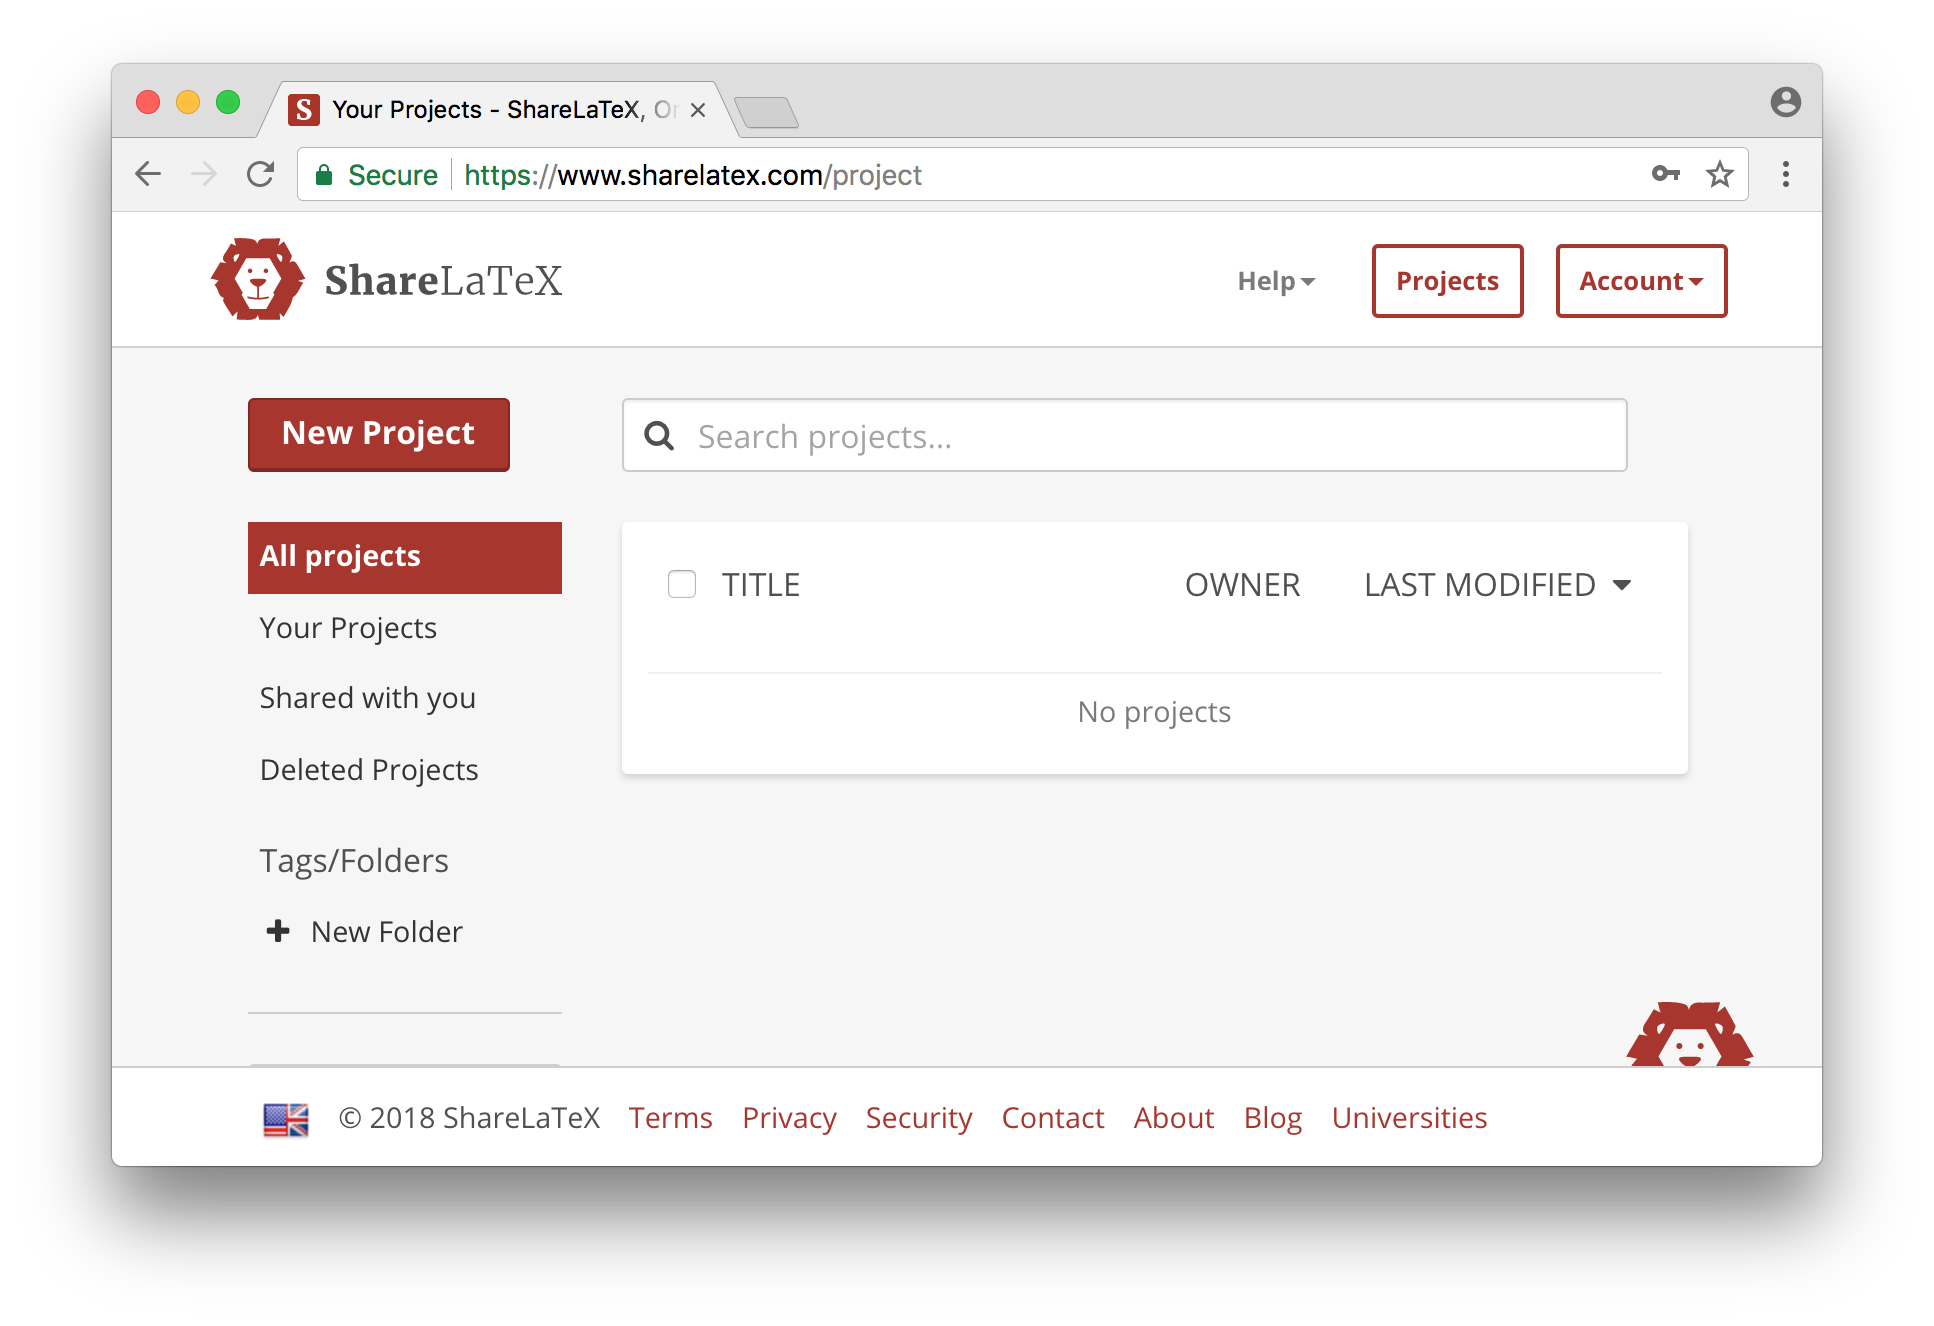
\includegraphics[width=.8\textwidth]{images/latex_login}


\paragraph{} Now click ``New Project'' and select ``View All''.

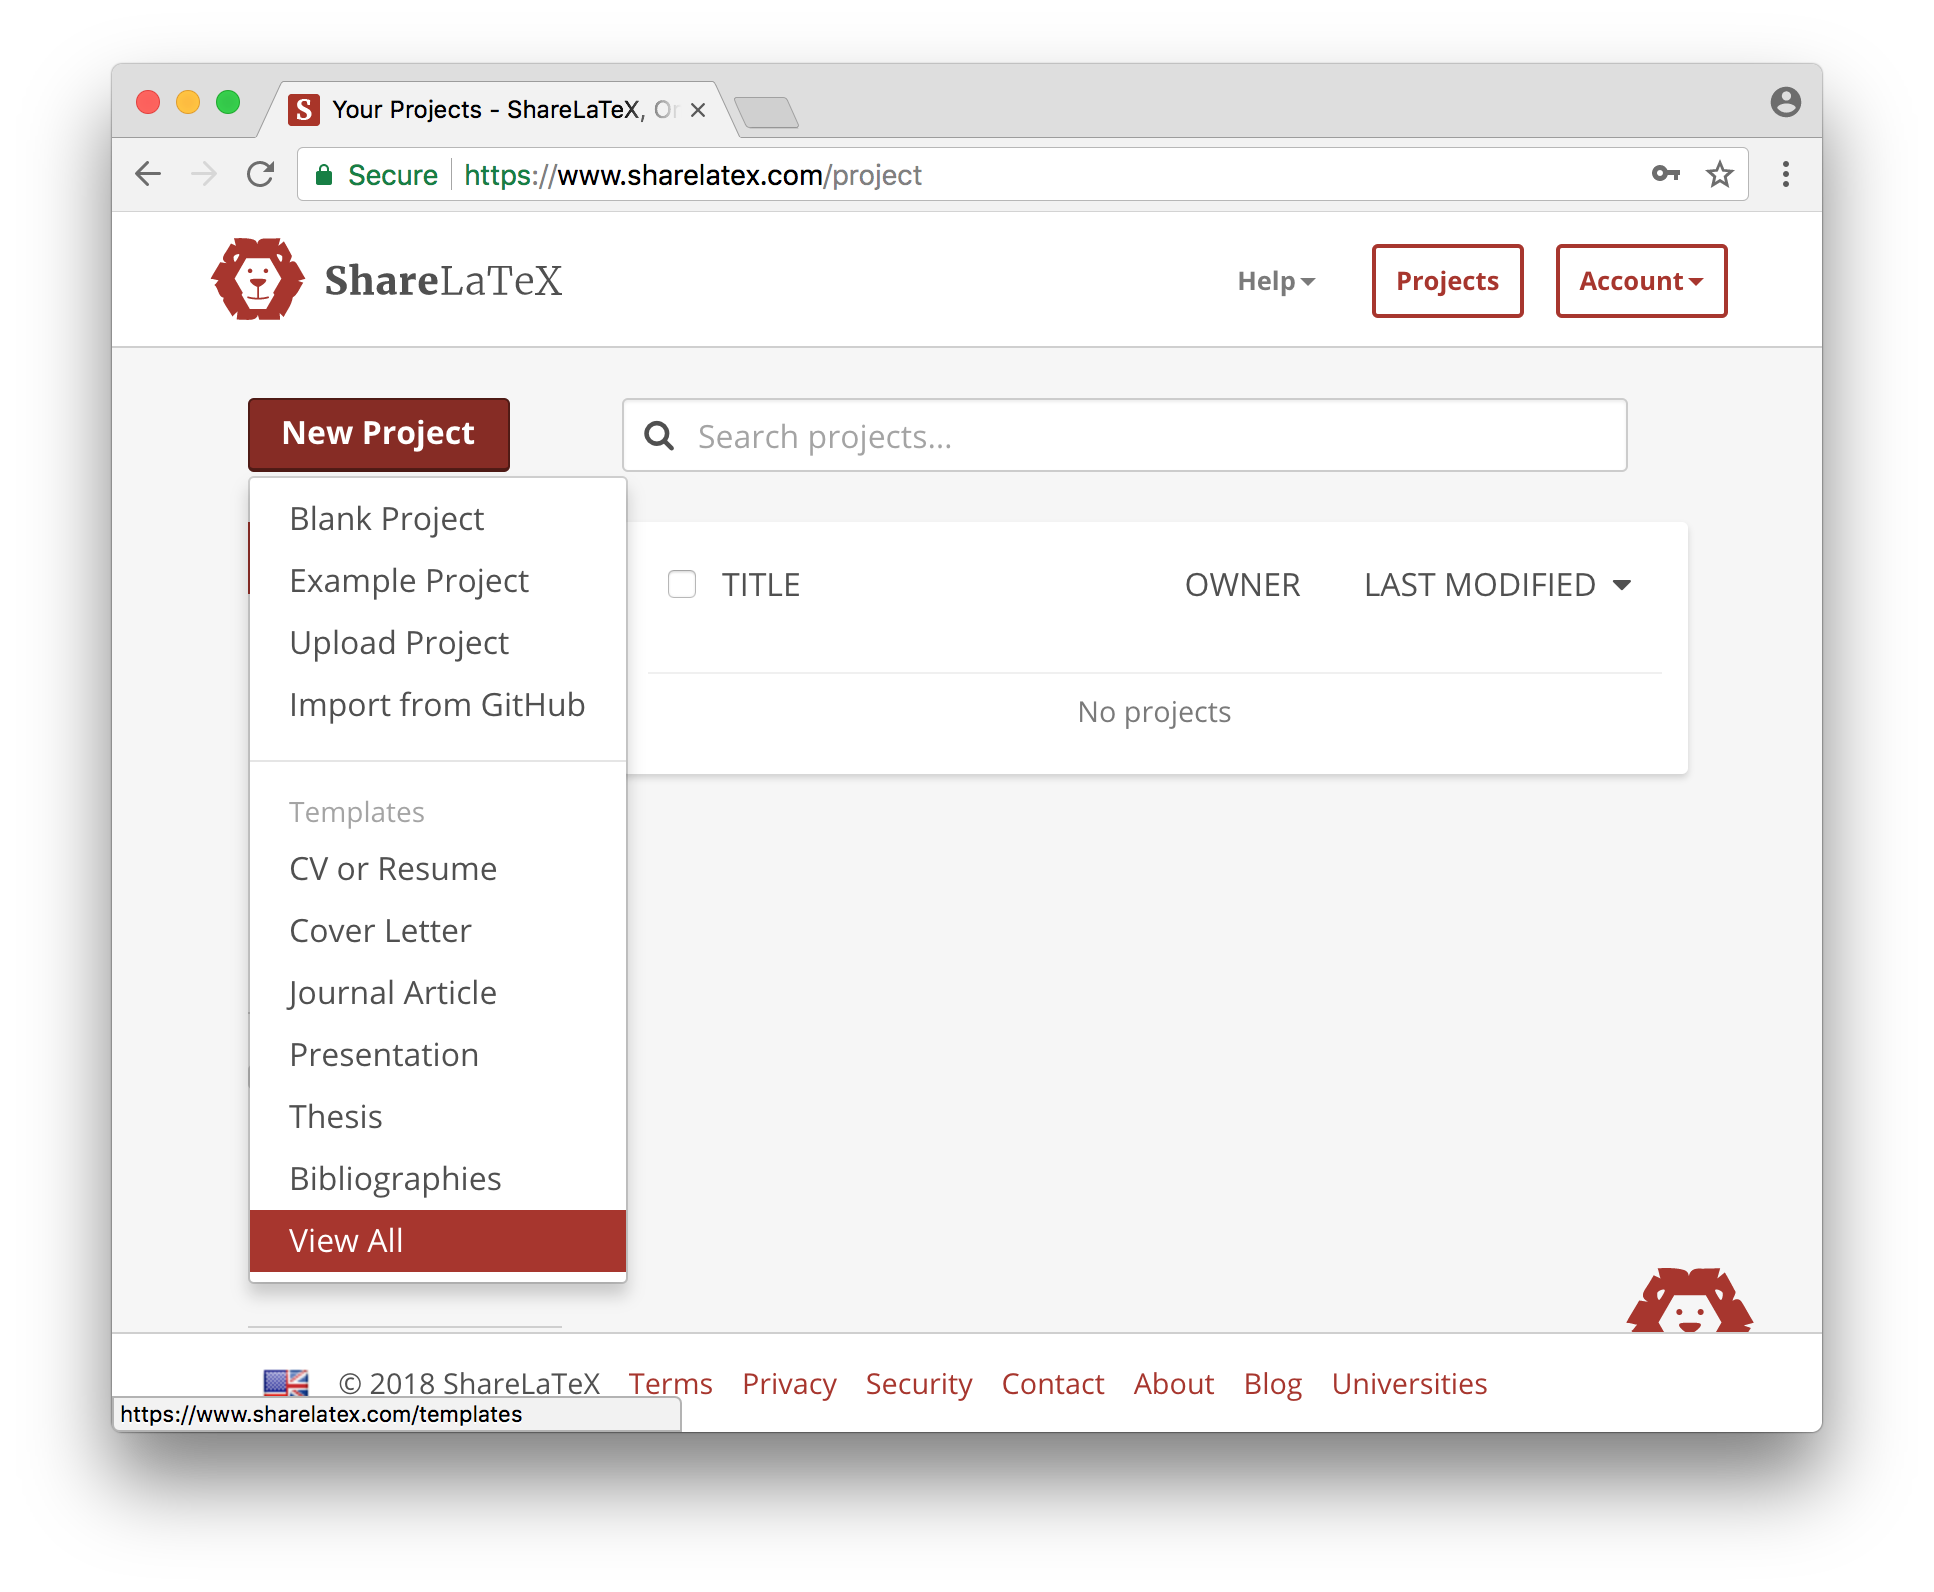
\includegraphics[width=.8\textwidth]{images/latex_new-project}

\paragraph{} Type ``Napier'' into the search box and you should see a suggestion for the Edinburgh Napier \LaTeX report template. Select the ``Edinburgh Napier Coursework Report'' option.

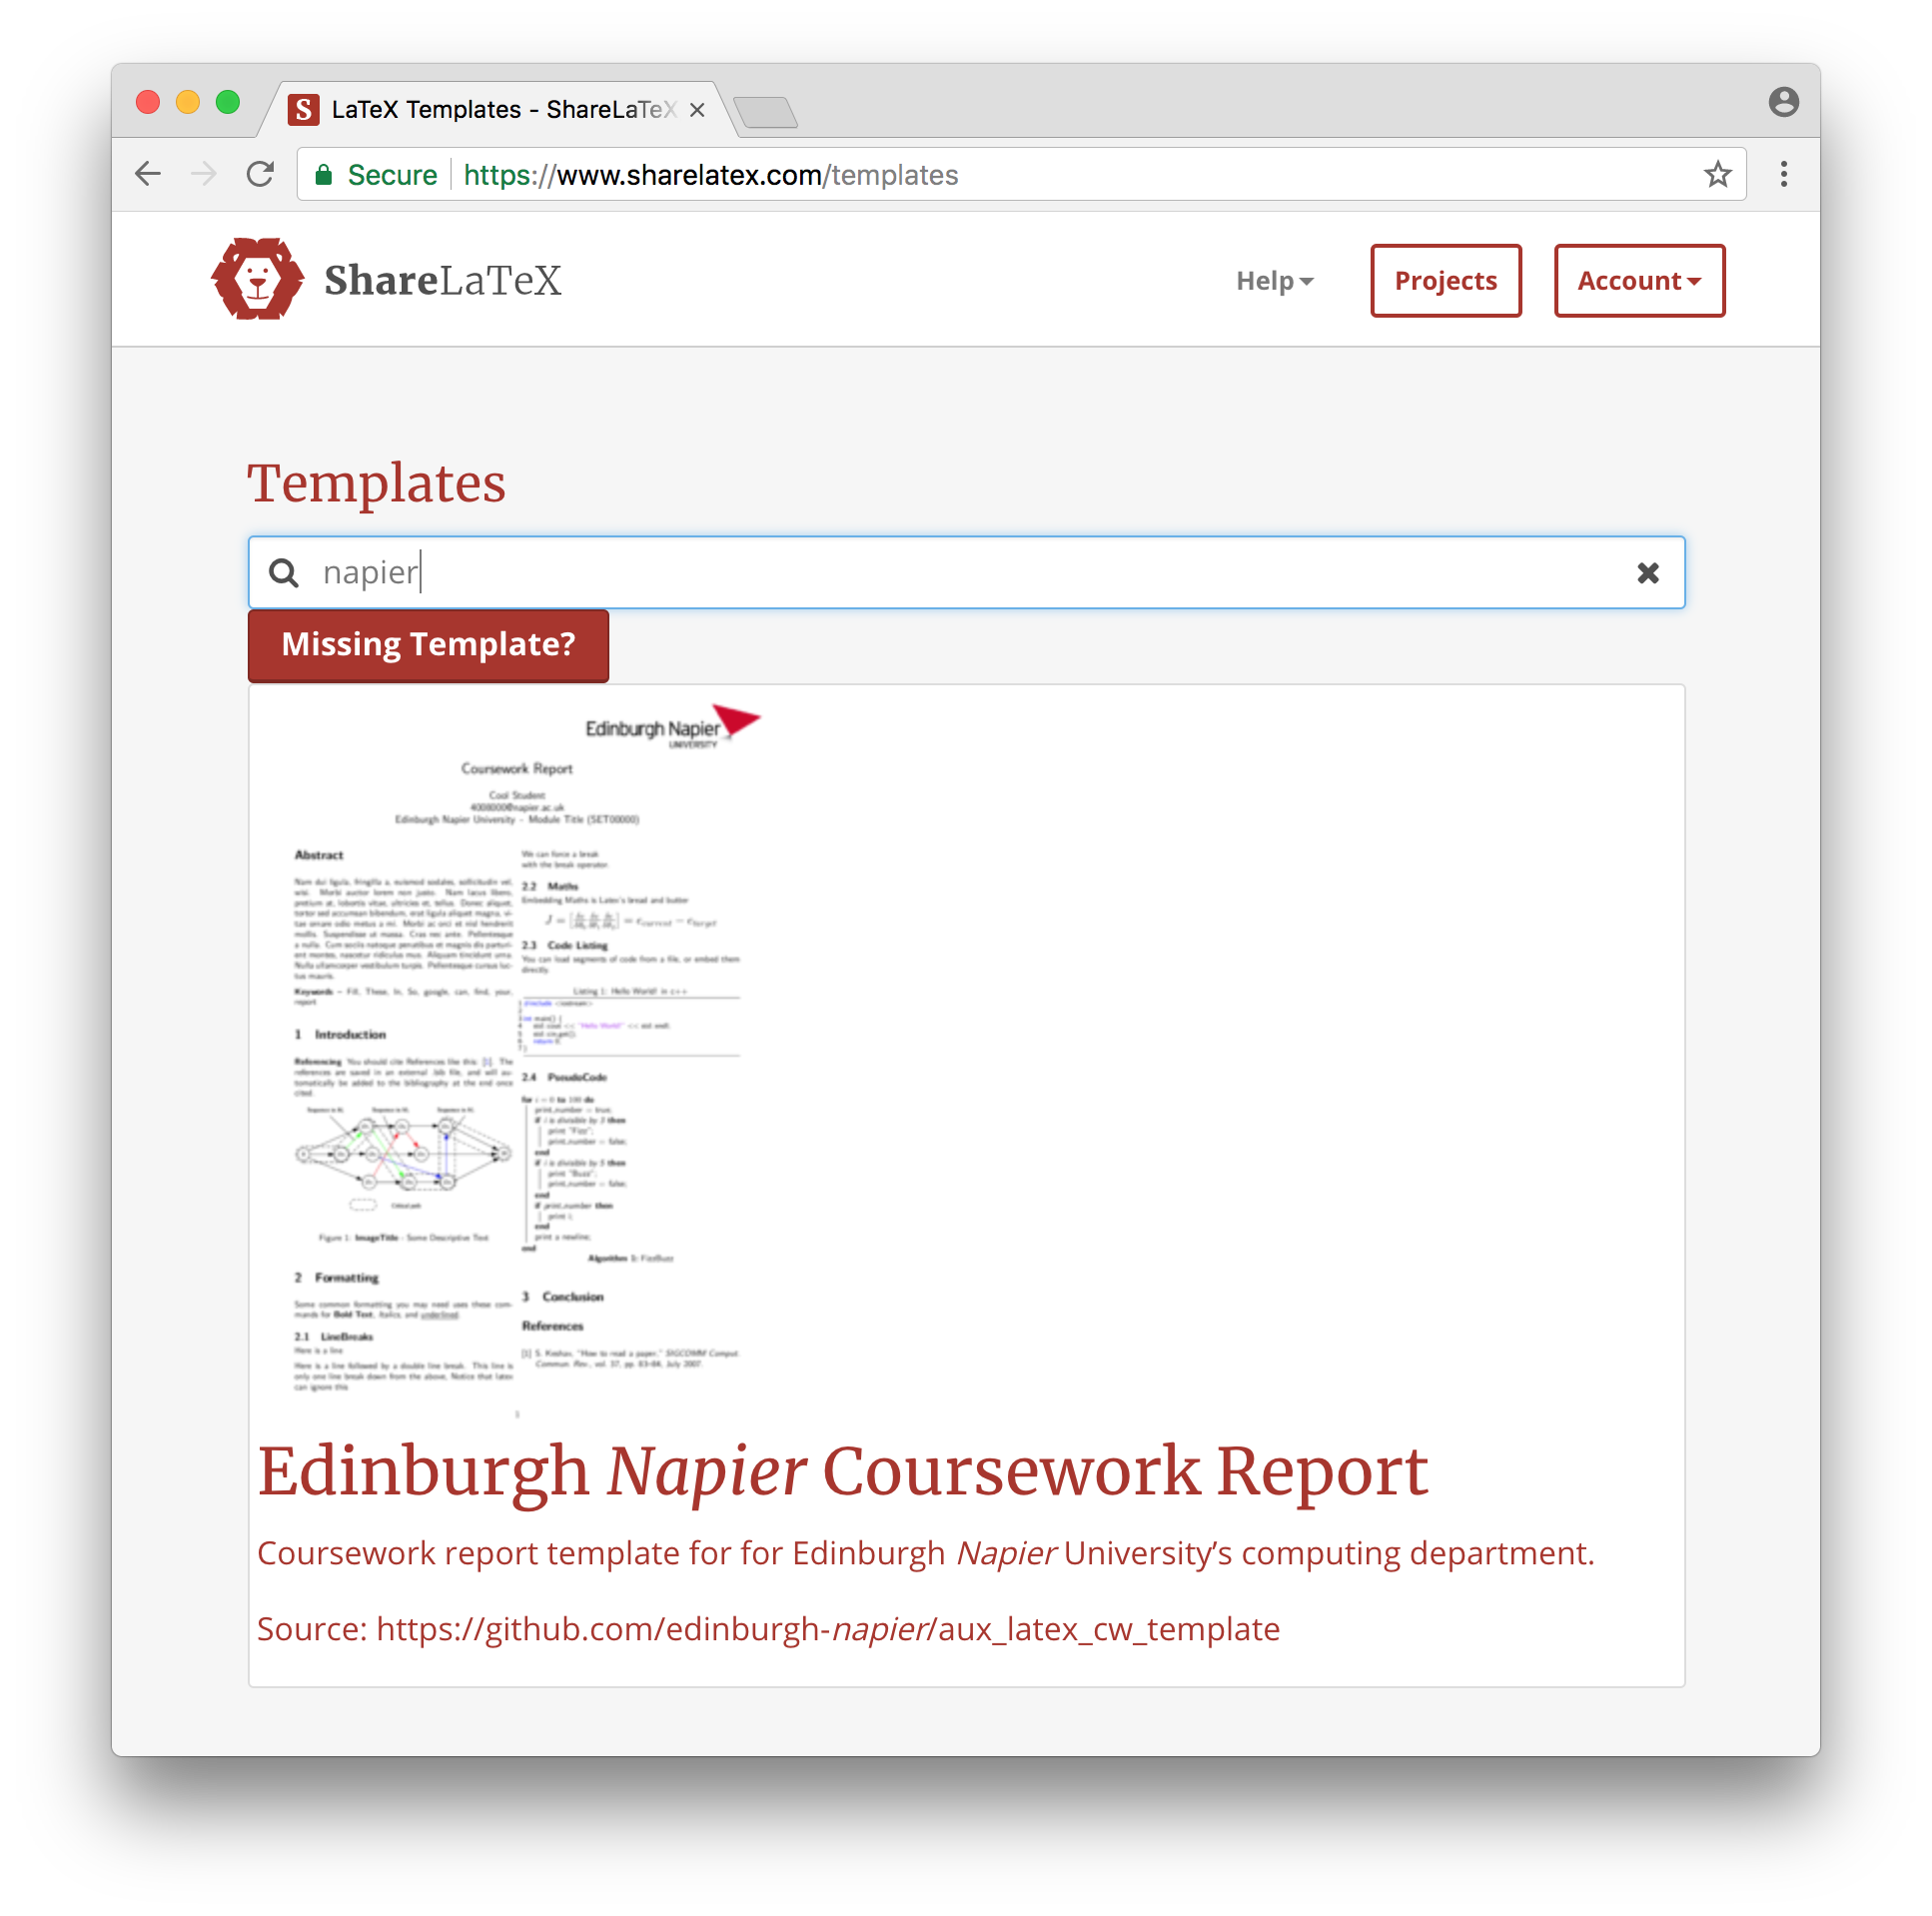
\includegraphics[width=.8\textwidth]{images/latex_enu-template}

\paragraph{} Select ``Open in ShareLatex'' and a new project will be created for you with the template already applied.

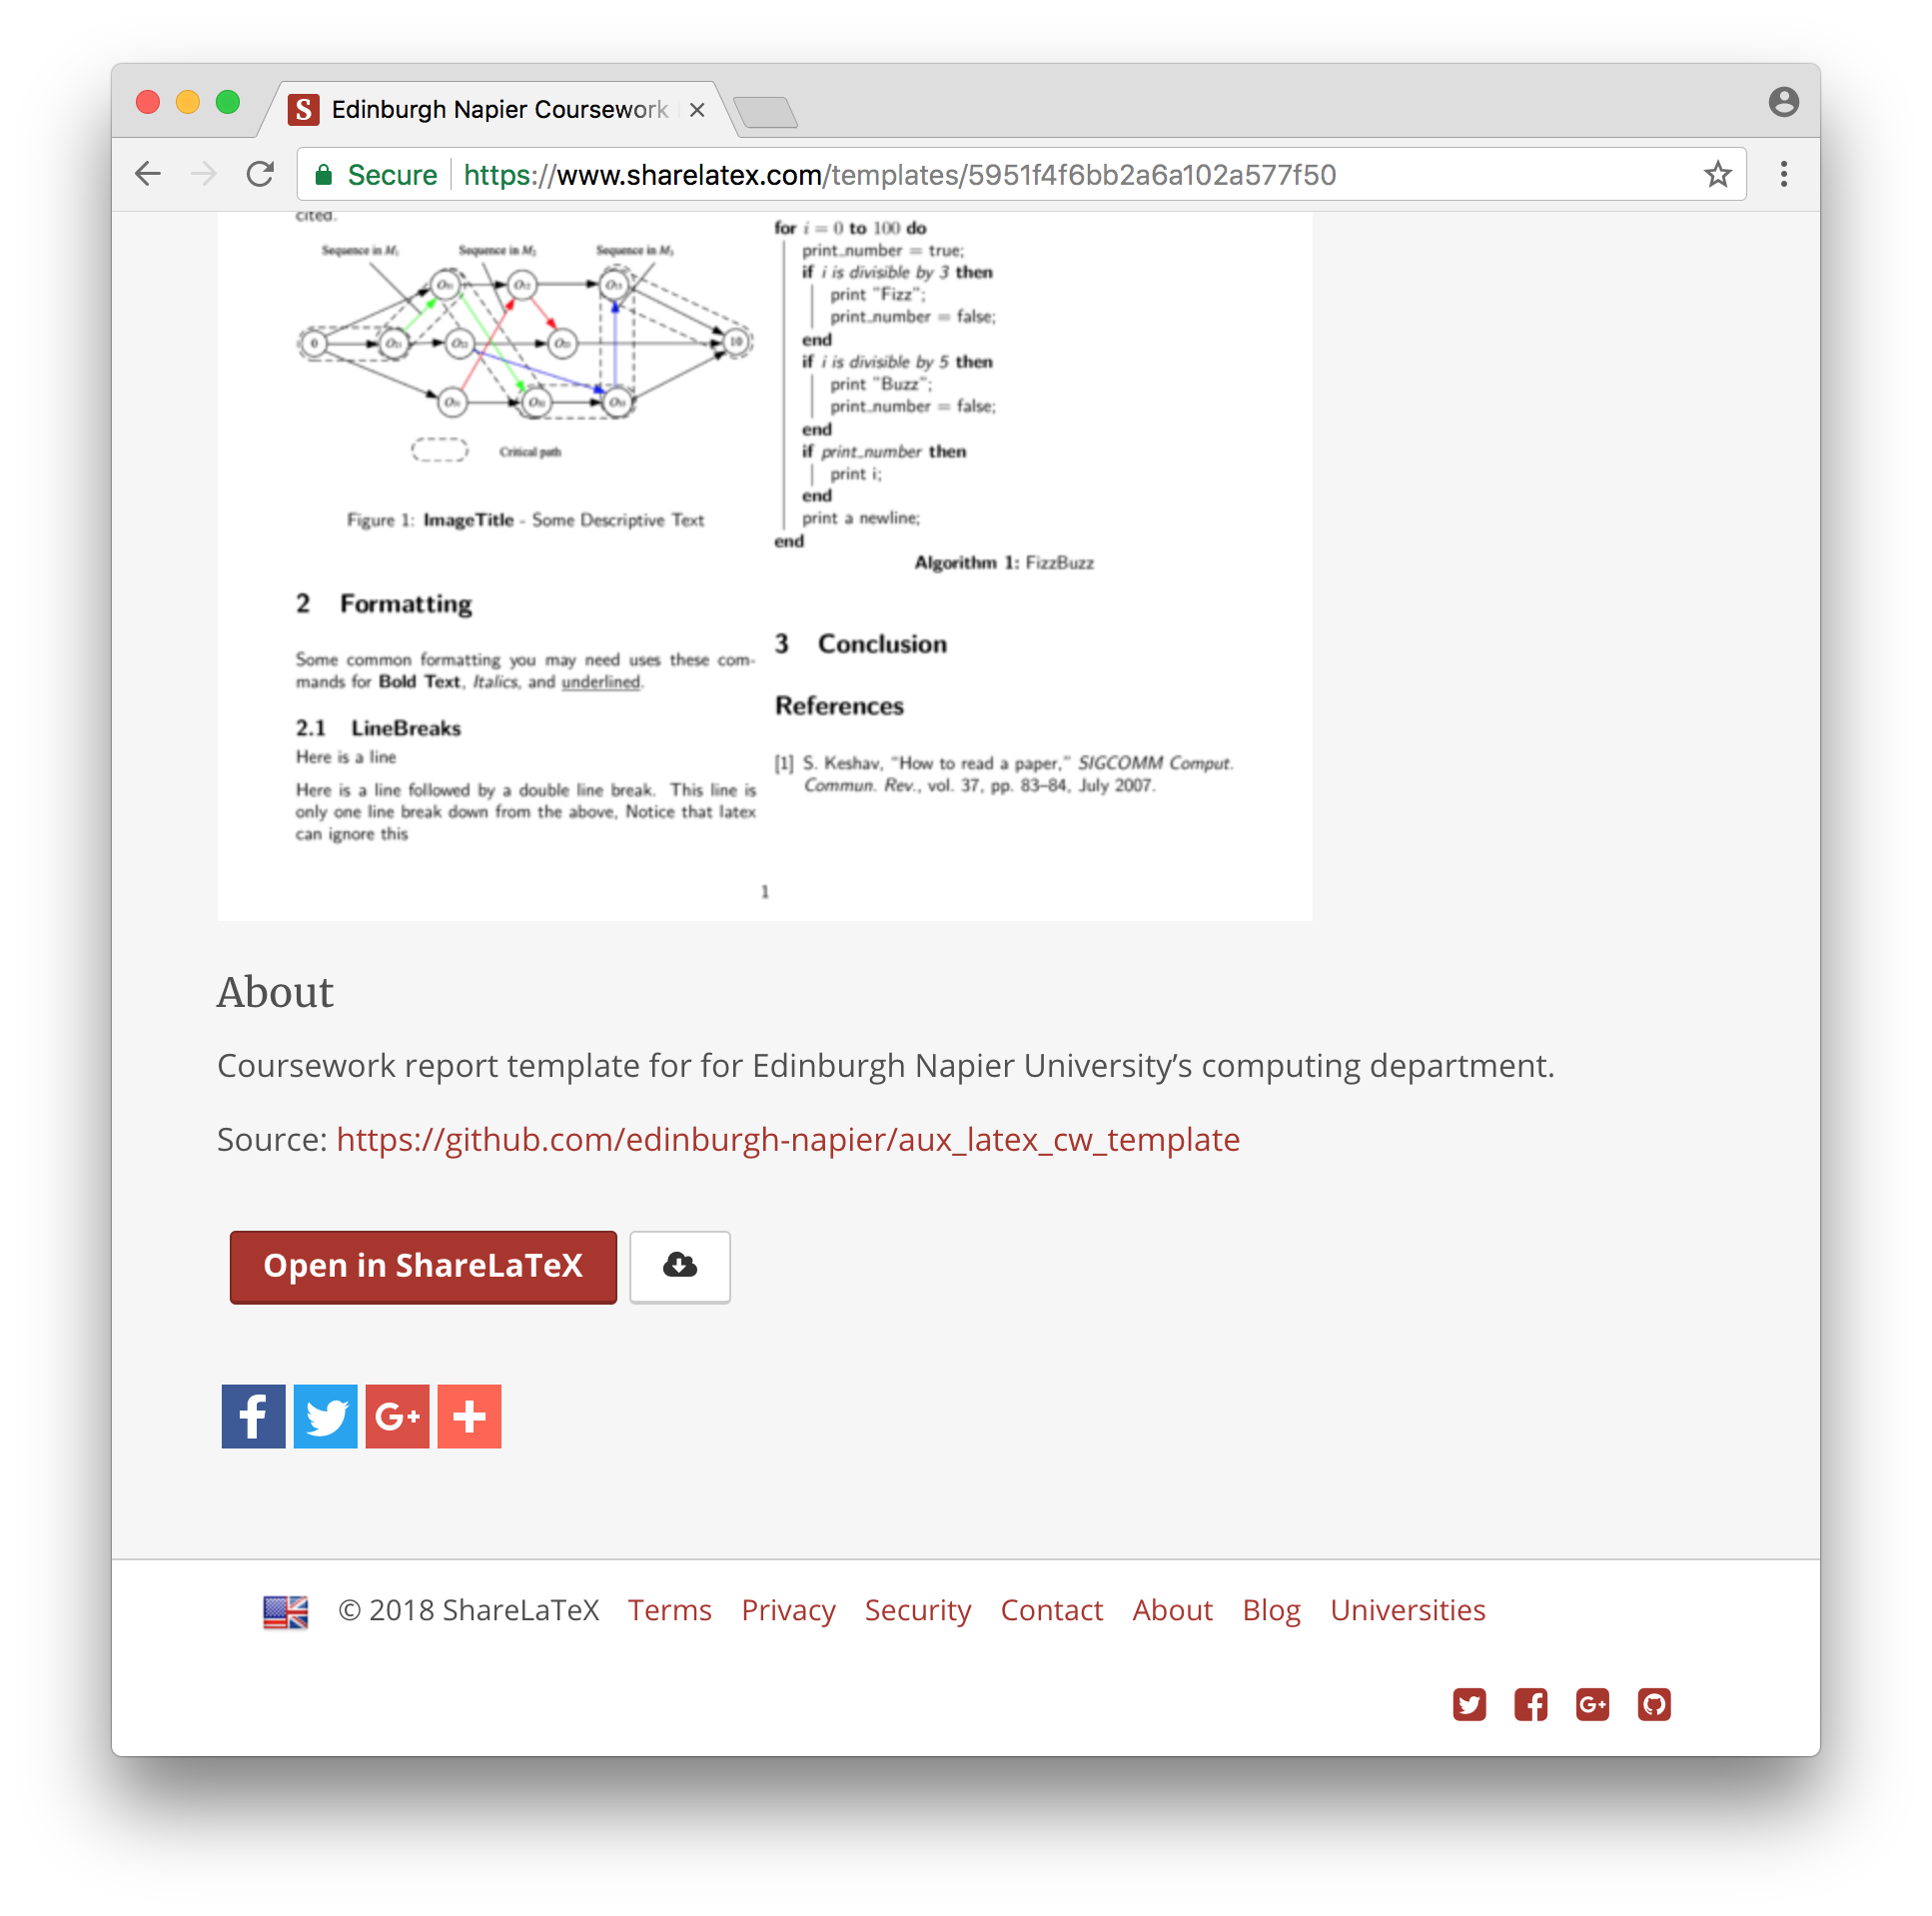
\includegraphics[width=.8\textwidth]{images/latex_open-in}


\paragraph{} On the left is a file manager for handling the different files that make up your document. The center is the text editor for writing the \LaTeX source. On the right is a preview of your generated PDF.

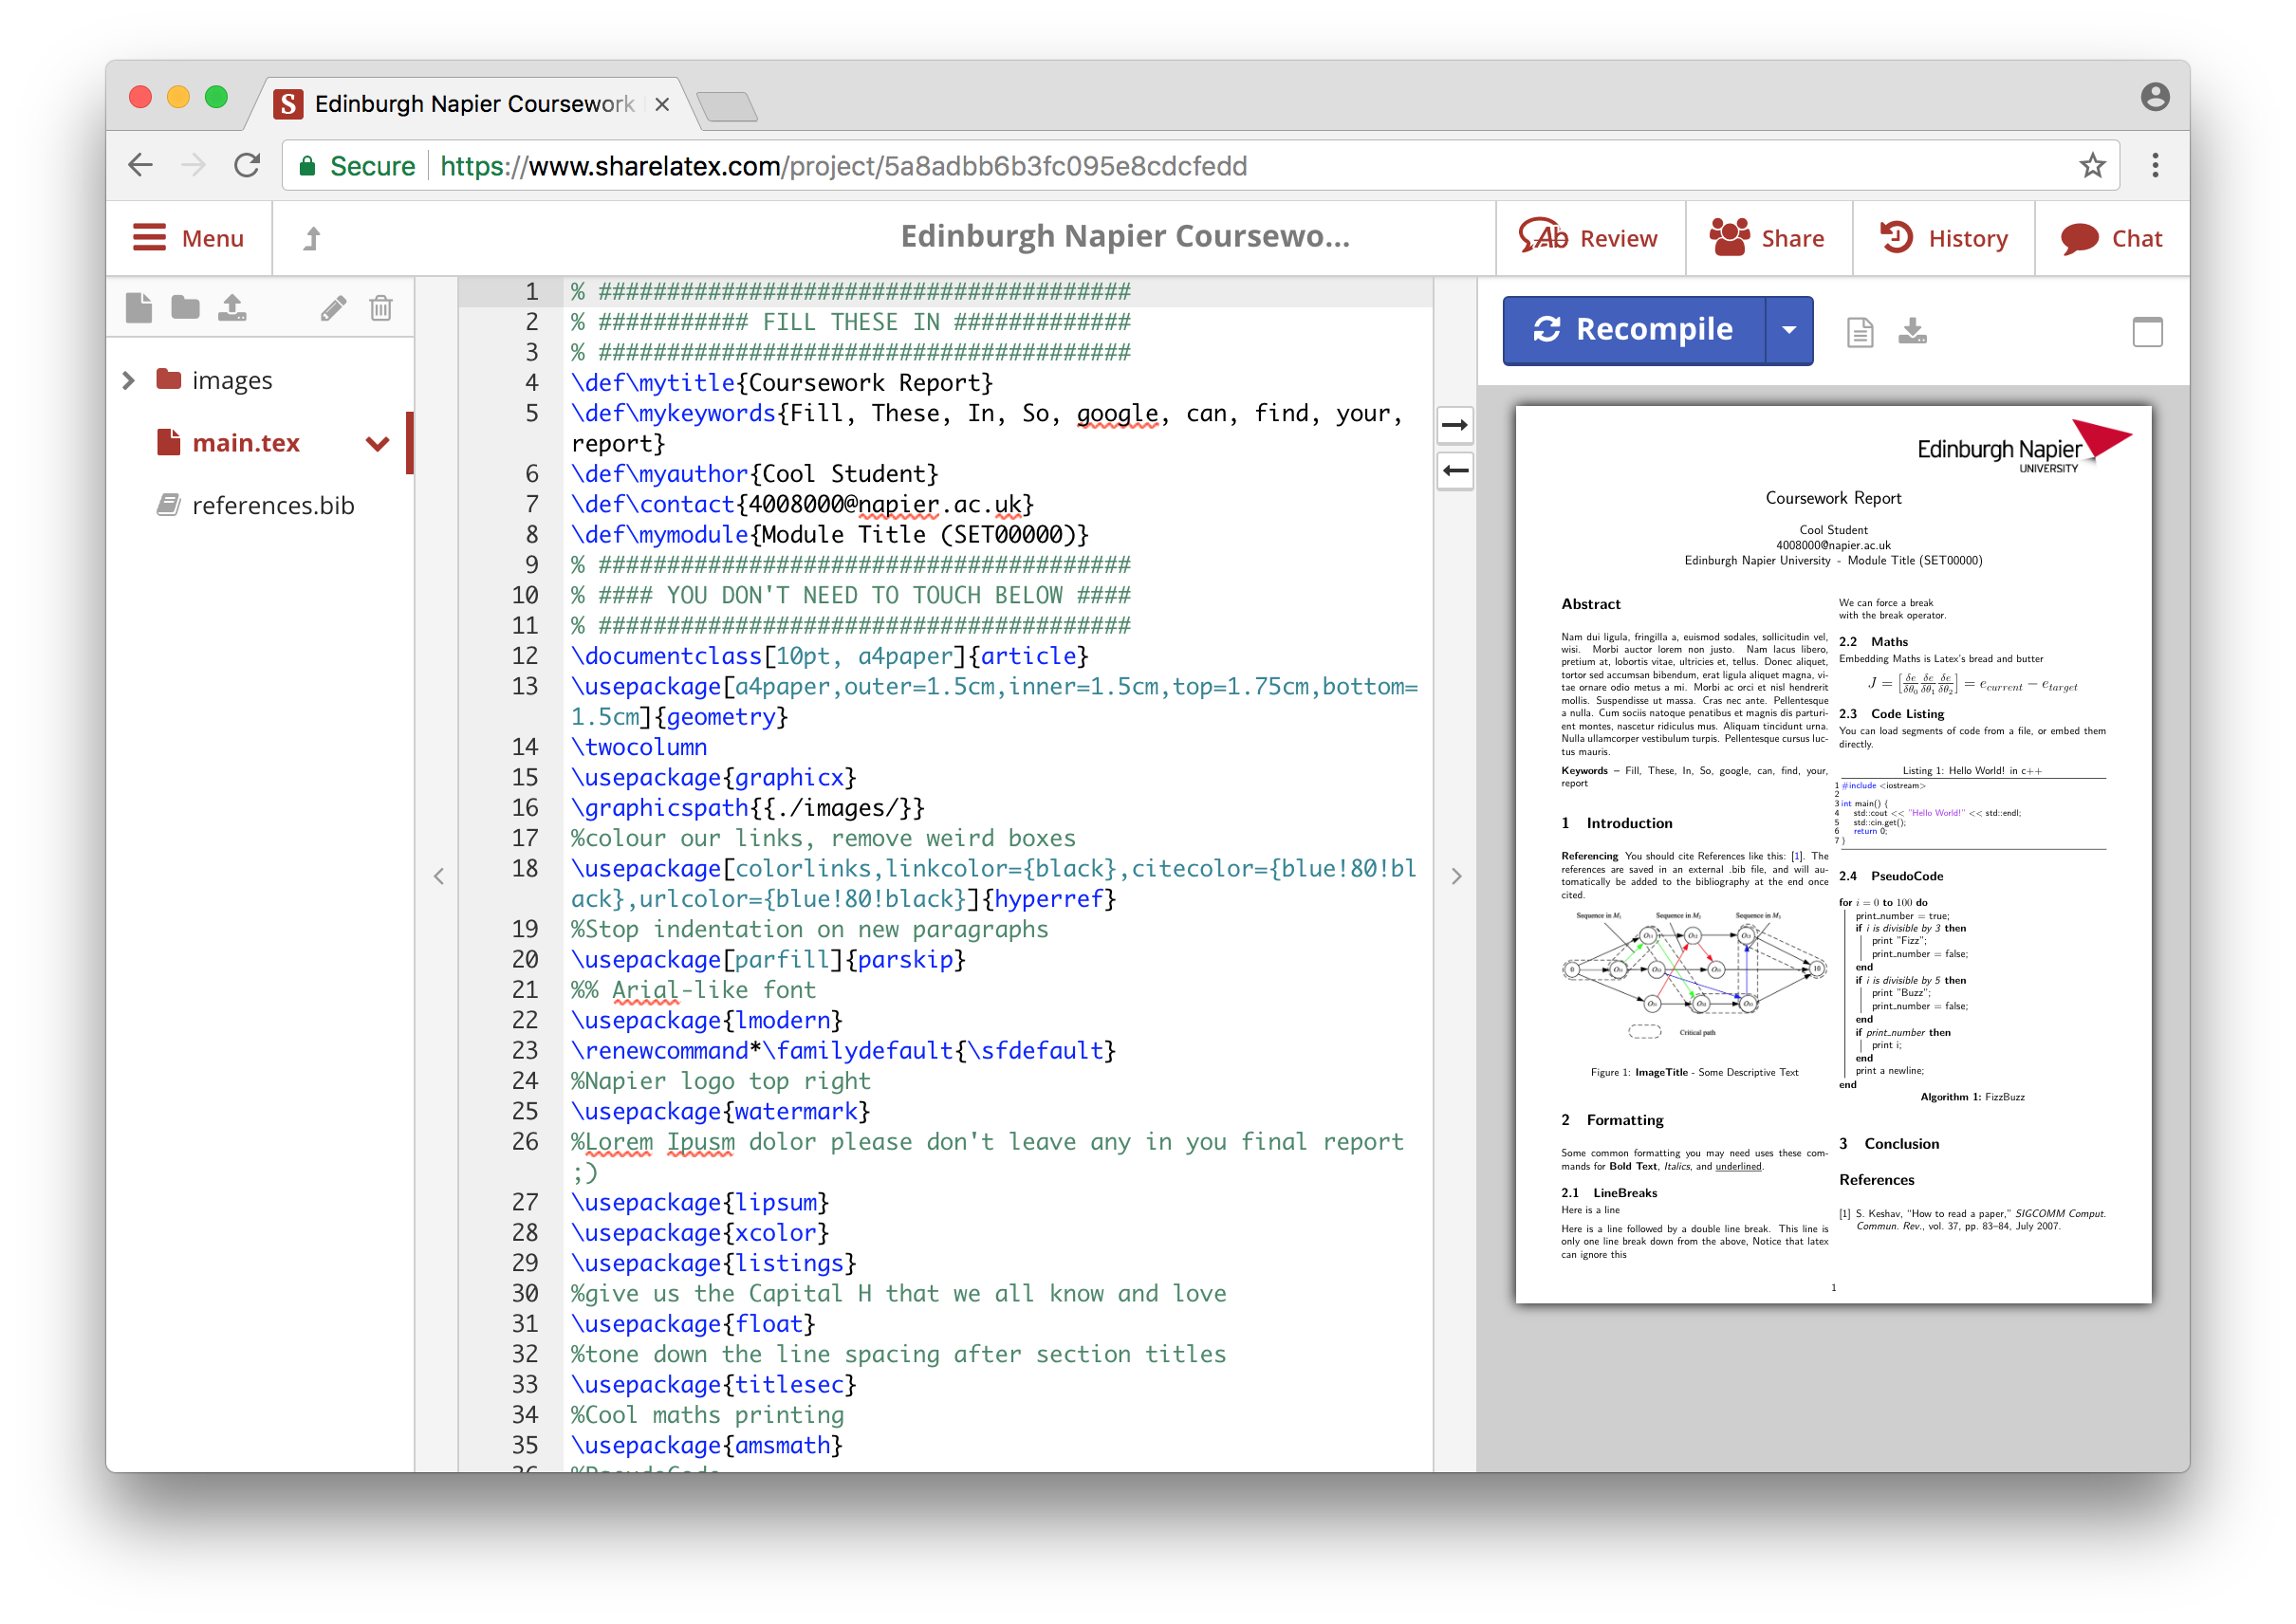
\includegraphics[width=.8\textwidth]{images/latex_ui}

\paragraph{} You can download this PDF at any time by hitting the download button:


\includegraphics[width=.2\textwidth]{images/latex_download-icon}

\paragraph{} Edit the following section of the \LaTeX file to fill in your own details:

\begin{lstlisting}
% #######################################
% ########### FILL THESE IN #############
% #######################################
\def\mytitle{Coursework Report}
\def\mykeywords{Fill, These, In, So, google, can, find, your, report}
\def\myauthor{Cool Student}
\def\contact{4008000@napier.ac.uk}
\def\mymodule{Module Title (SET00000)}
\end{lstlisting}

\paragraph{} Your actual report content starts further down the page at this point:

\begin{lstlisting}
% #######################################
% ########### START FROM HERE ###########
% #######################################
\end{lstlisting}

\paragraph{} You can now delete the example contents, everything between the line that reads:

\begin{lstlisting}
    \begin{abstract}
\end{lstlisting}

which should be line 77, and the line that reads:

\begin{lstlisting}
    \section{Conclusion}
\end{lstlisting}

which should be line 146. We should be left with a section that looks like this:

\begin{lstlisting}
% #######################################
% ########### START FROM HERE ###########
% #######################################
\begin{document}
	\maketitle




\bibliographystyle{ieeetr}
\bibliography{references}

\end{document}
\end{lstlisting}



\paragraph{} We can now start to add our own content. A good place to start is to add in the various section headings that the coursework descriptor asks for, e.g. 

\begin{lstlisting}
% #######################################
% ########### START FROM HERE ###########
% #######################################
\begin{document}
	\maketitle

\section{Introduction}


\section{Software Design}


\section{Implementation}


\section{Critical Evaluation}


\section{Personal Evaluation}


\bibliographystyle{ieeetr}
\bibliography{references}
		
\end{document}
\end{lstlisting}


\paragraph{} Our document should now look something like this:


\includegraphics[width=.8\textwidth]{images/latex_preview}

\paragraph{} You can now start writing your text into the sections that we've just outlined. For now just write the text that you need in your report. If you want to get more fancy then there is a whole host of \LaTeX features that you can take advantage of but that is an exercise for you to pursue. Remember however that one of the powers of \LaTeX is that it free us from worrying too much about what things look like, the tool takes care of that for the most part, and in this case we have a template\footnote{Don't edit the template; the idea of using \LaTeX with a template is to get consistency of presentation across multiple documents}. This allows us to concentrate on just writing the content.


\section{Going Further}
\paragraph{} \LaTeX is an entire typesetting language that is used to typeset everything from academic research papers through to entire books. It has a reputation for consistent and high-quality typesetting. This means that there is a lot more to the capabilities of \LaTeX than we've covered here. 

%\backmatter

\bibliographystyle{plain}

\bibliography{workbook}

\end{document}

%\begin{framed}
%HELLO
%\end{framed}


%\begin{lstlisting}
%\end{lstlisting}


%\includegraphics[width=.8\textwidth]{images/}
